% Generated by thesis/ch7/exp2/networks.py -- do not edit by hand.
\begin{sidewaysfigure}
  \centering
  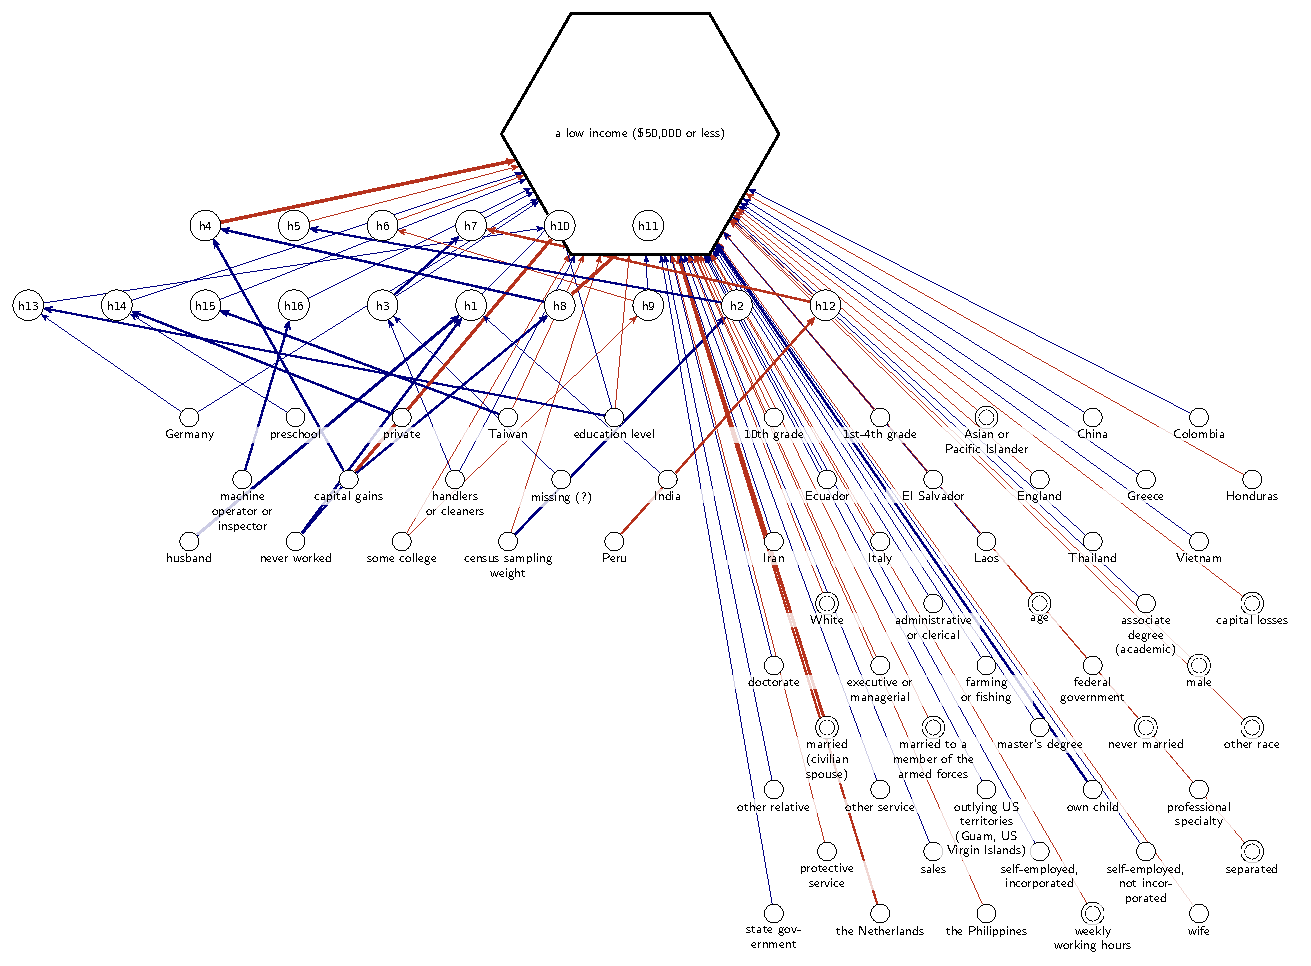
\includegraphics[width=\textheight,height=0.78\textwidth,keepaspectratio]{figures/exp2/networks/adult-s2-raw}
  \caption{Adult, seed 2 (adult-s2): the network as trained, before any explanation, in full. Inputs at the bottom (every input column its own node), hidden units by depth, the output at the top; 60 of 107 input columns are connected, with 16 hidden units and 91 enabled connections. Blue: positive weight (raises the score); red: negative weight (lowers it); thicker: larger weight. Orange outline and up arrow: raises the final prediction; teal and down arrow: lowers it; grey and double arrow: depends. Not used (no connection; 47 columns): missing (?), local government, without pay, 11th grade, high-school graduate, professional school degree, 12th grade (no diploma), 5th-6th grade, 7th-8th grade, 9th grade, associate degree (vocational), bachelor's degree, divorced, married, spouse absent, widowed, technical support, transport or moving, armed forces, craft or repair, private household service, not in a family, unmarried, American Indian or Eskimo, Black, missing (?), Cambodia, France, Guatemala, Haiti, Hong Kong, Hungary, Canada, Ireland, Jamaica, Japan, Mexico, Nicaragua, Poland, Portugal, Puerto Rico, Scotland, 'South' (as recorded), Trinidad and Tobago, the United States, Yugoslavia, Cuba and Dominican Republic.}
  \label{fig:exp2-net-adult-s2-raw}
\end{sidewaysfigure}
